\section{Projekt interfejsu użytkownika}

W celu zwiększenia czytelności prototypów interfejsu użytkownika
zostały one zamieszczone w orientacji pionowej, co umożliwiło
zwiększenie ich rozmiaru i czcionki na nich do przystępnych rozmiarów.

\subsection{Logowanie}

\begin{figure}[H]
	\centering
        \vfill
        \noindent
        \makebox[\textwidth]{
          
\includegraphics[width=0.8\textheight,angle=270]{img/screens/logowanie.png}
        }
	\caption{Ekran logowania}
\end{figure}

\subsection{Wyszukiwanie zasobu}

\begin{figure}[H]
	\centering
        \vfill
        \noindent
        \makebox[\textwidth]{
          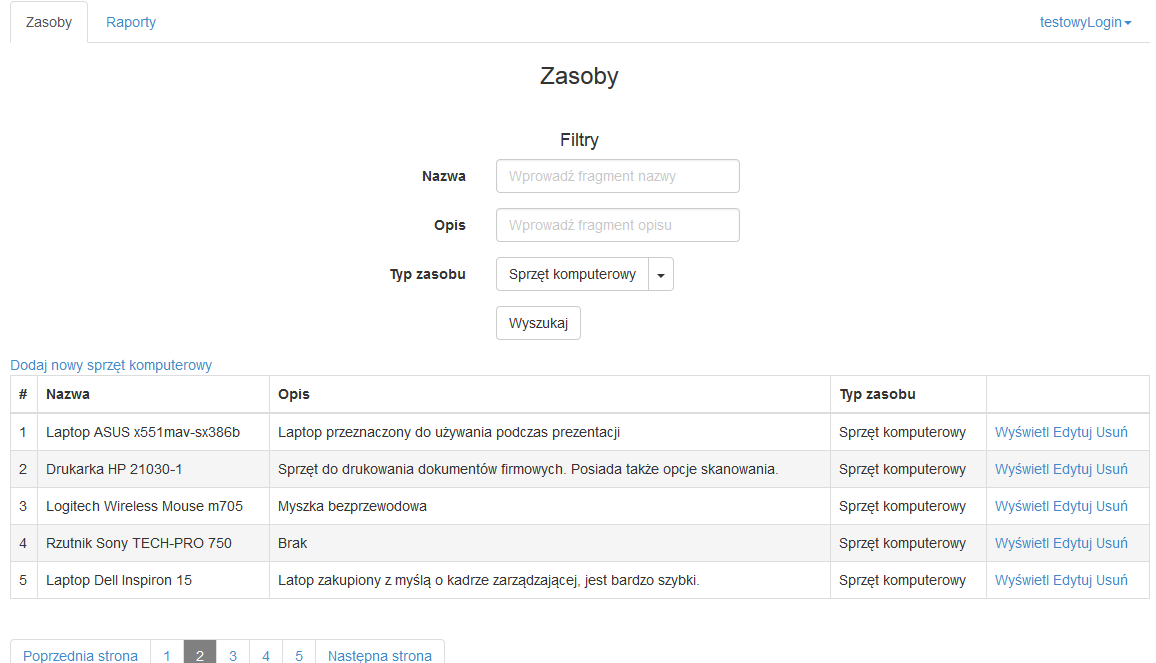
\includegraphics[width=0.8\textheight,angle=270]{img/screens/wyszZasob.png}
        }
	\caption{Ekran wyszukiwania zasobów}
\end{figure}

\subsection{Dodawanie sprzętu komputerowego}
\begin{figure}[H]
	\centering
        \vfill
        \noindent
        \makebox[\textwidth]{
          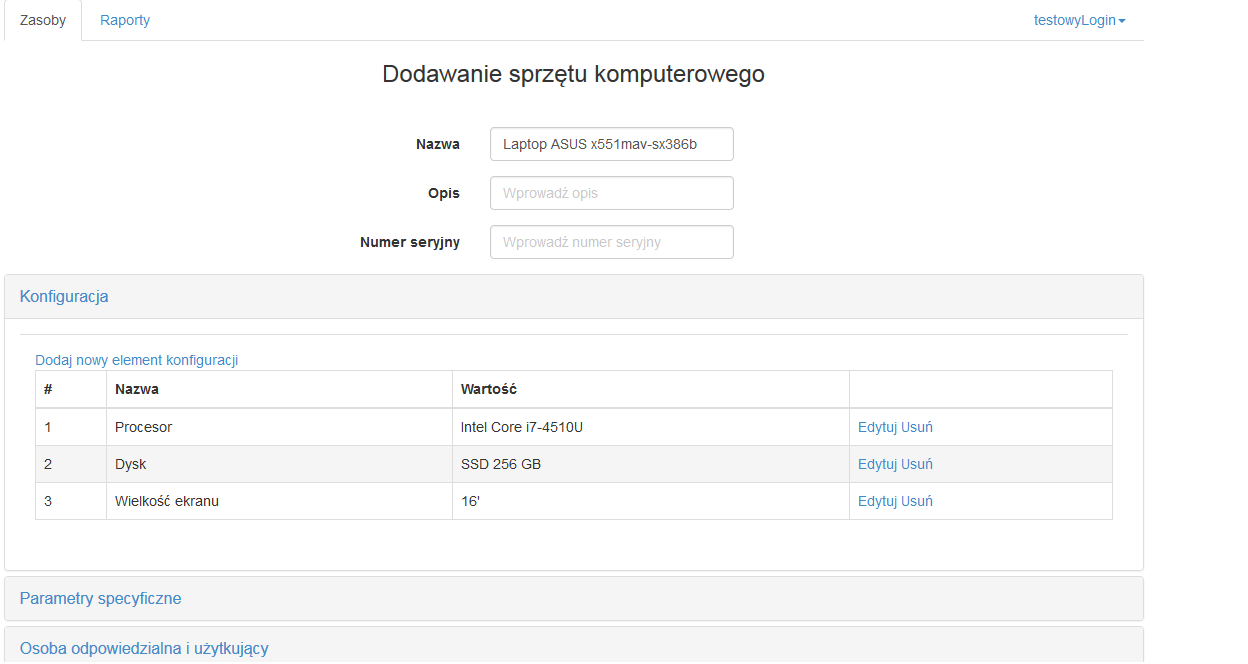
\includegraphics[width=0.8\textheight,angle=270]{img/screens/dodawanieSprzetuKomputerowego.png}
        }
	\caption{Ekran dodawania sprzętu komputerowego}
\end{figure}

\subsection{Zapisanie informacji o użytkowniku oprogramowania}
\begin{figure}[H]
	\centering
        \vfill
        \noindent
        \makebox[\textwidth]{
          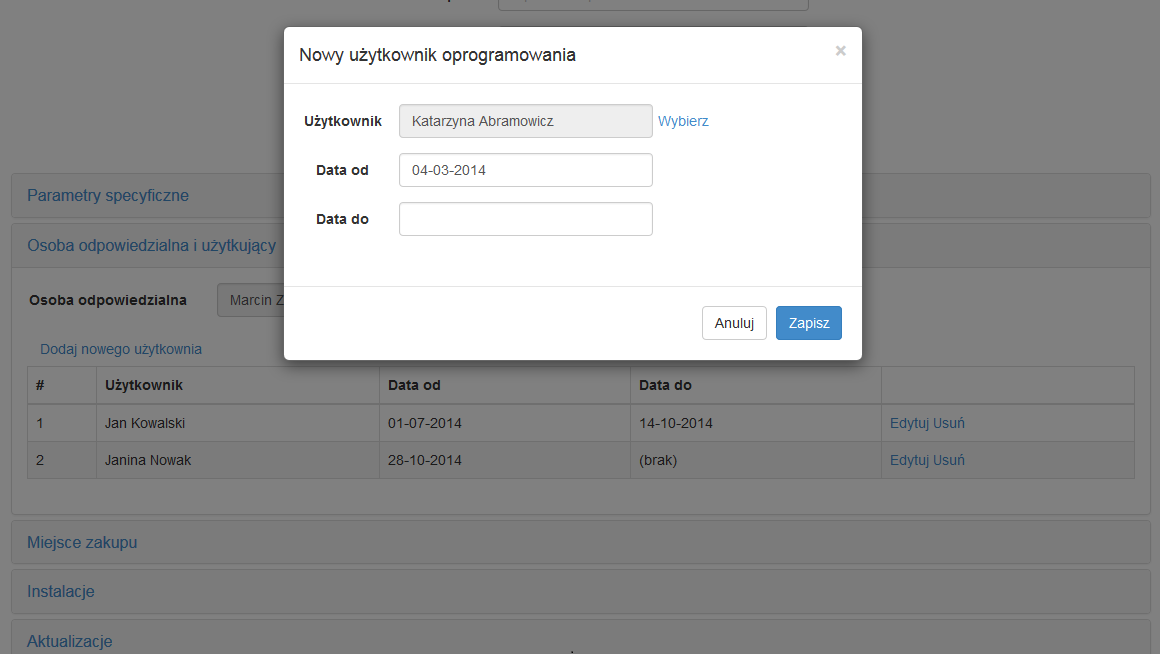
\includegraphics[width=0.8\textheight,angle=270]{img/screens/nowyUzytkownikOprogramowania.png}
        }
	\caption{Dodawanie użytkownika oprogramowania}
\end{figure}

\subsection{Rejestracja miejsca zakupu literatury lub zasobu literaturowego}
\begin{figure}[H]
	\centering
        \vfill
        \noindent
        \makebox[\textwidth]{
          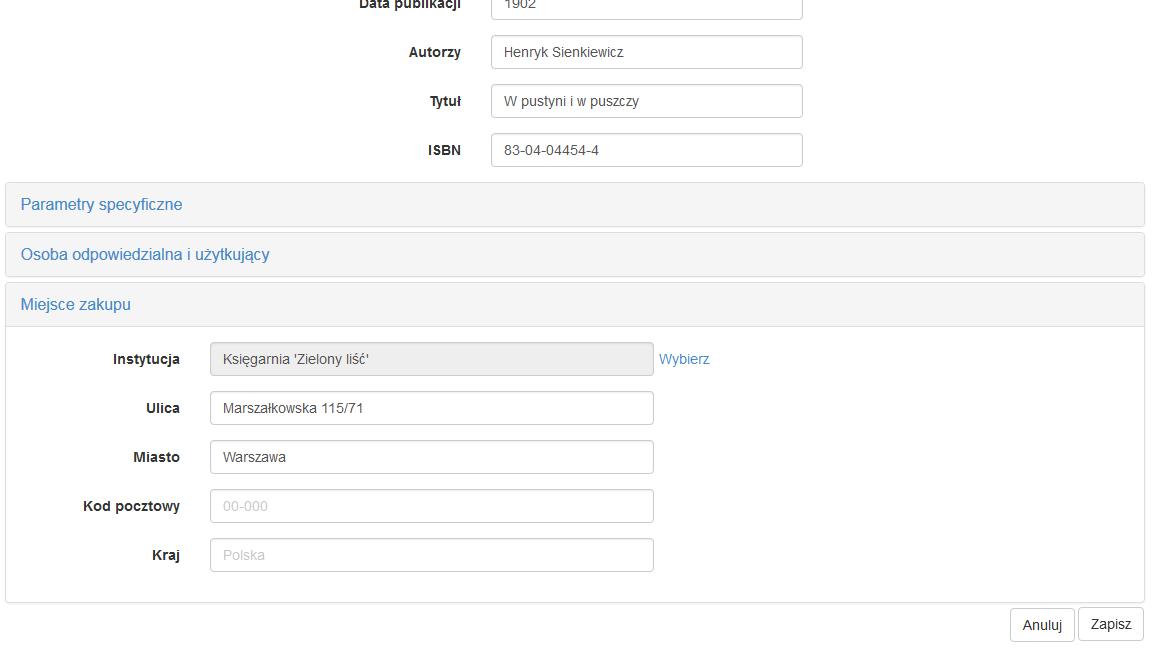
\includegraphics[width=0.8\textheight,angle=270]{img/screens/miejsceZakupuLiteratura.png}
        }
	\caption{Edycja informacji na temat miejsca zakupu}
\end{figure}

\subsection{Edytowanie historii napraw sprzędu}
\begin{figure}[H]
	\centering
        \vfill
        \noindent
        \makebox[\textwidth]{
          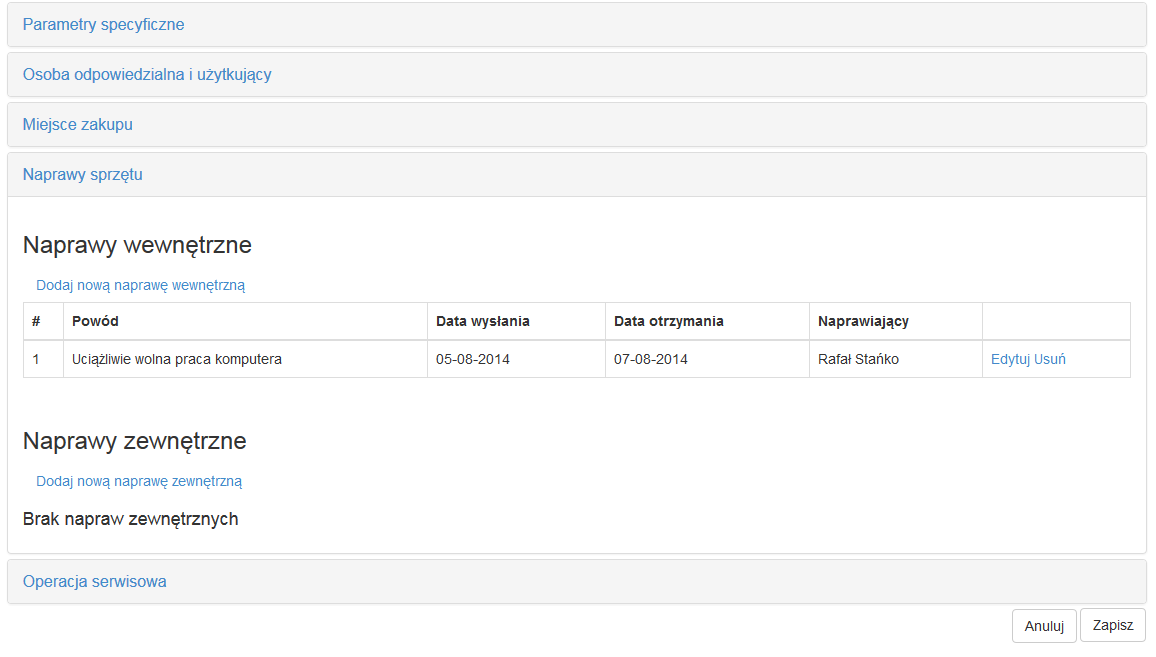
\includegraphics[width=0.8\textheight,angle=270]{img/screens/naprawyWew.png}
        }
	\caption{Modyfikacja historii napraw sprzętu}
\end{figure}

\subsection{Prezentacja ilosci zakupionych zasobow w dzialach}
\begin{figure}[H]
	\centering
        \vfill
        \noindent
        \makebox[\textwidth]{
          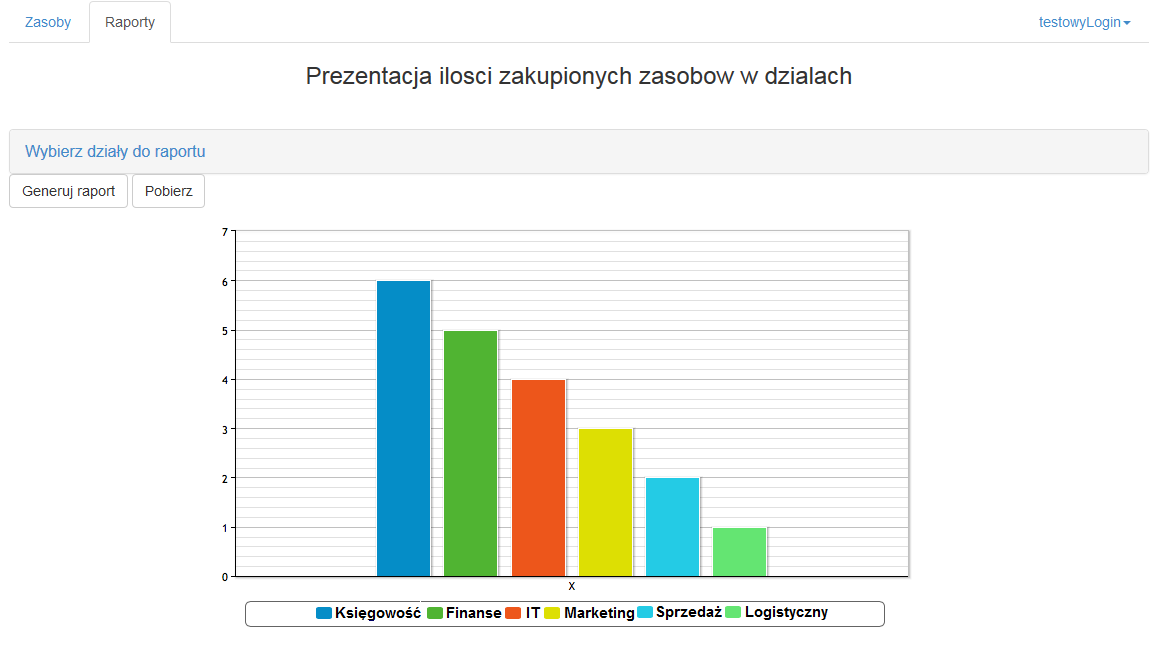
\includegraphics[width=0.8\textheight,angle=270]{img/screens/raport.png}
        }
	\caption{Przykładowy raport - prezentacja ilosci zakupionych zasobow w dzialach}
\end{figure}
